\clearpage
\section{Multirobot problem}
\subsection{Problem definition and states}

The different between single robot problem and multi robot problem is, every robot take turns to make actions, and it needs collision detection. In thiscase, we decide the a whole state for all the $k$ robots, like this:



$$\begin{pmatrix}
  x_0 & y_0 \\
  x_1 & y_1 \\
  \vdots & \vdots \\	
  x_{k-1} & y_{k-1}
 \end{pmatrix}$$
 
 However, this is not enough for the states. We still one parameter, which the turn of the robot. This parameter is not necessary, which means you can still solve the problem without it in the state. However, returning all the possible states of $k$ can be very redundant and time consumming for latter searching. If I have k robot, and five actions (4 directions plus not moving), the upper bound of states would be $5^k$. It is like giving too much options more next step, while I am not making any decision. 


\subsection{Code implementation}




\subsubsection{getSuccessors}

\textbf{Line 4:} Iterate through all the 5 possible actions (4 directions plus not moving).


\textbf{Line 6-7:} Initiate the coordinates for the successor's state, noted that only the robot in turn can take action here.


\textbf{Line 11-13:} Construct the successor with new coordinates, and new cost based on whether it moves, and also keep looping the turn through $R$ robots.


\begin{lstlisting}[numbers=left]
public ArrayList<SearchNode> getSuccessors() {
  ArrayList<SearchNode> successors = new ArrayList<SearchNode>();
  Integer[] xNew = new Integer[R], yNew = new Integer[R];
  for (int[] action : actions) {
    for (int r = 0; r < R; r++) {
      xNew[r] = robots[r][0] + action[0] * (r == turn ? 1 : 0);
      yNew[r] = robots[r][1] + action[1] * (r == turn ? 1 : 0);
    }
    if (maze.isLegal(xNew[turn], yNew[turn])
        && noCollision(xNew, yNew)) {
      SearchNode succ = new MultirobotNode(xNew, yNew, getCost()
          + Math.abs(action[0]) + Math.abs(action[1]),
          (turn + 1) % R);
      successors.add(succ);
    }
  }
  return successors;
}
\end{lstlisting}



\subsubsection{Ohter methods}
Node constructor, it initiates the positions of robots iteratively.

\begin{lstlisting}[numbers=left]
public MultirobotNode(Integer[] x, Integer[] y, double c, int t) {
  robots = new int[R][2];
  for (int i = 0; i < R; i++) {
    this.robots[i][0] = x[i];
    this.robots[i][1] = y[i];
  }
  turn = t;
  cost = c;
}
\end{lstlisting}

\textbf{Line 20-28:} After poping the node, we check for two condition. One is if it is the goal, we simply return the solution path and terminate the search. Antoher condition is, if the node has been visited before, we don't push it into \emph{frontiers} unless it has shorter cost than before.

\textbf{Line 29-35:} Get the successors of currrent node, and push those un-visited nodes or node has shorter cost than before, into the \emph{frontiers}.



\subsection{Output demonstration}
I use Simplex Noise to generate the maze.\footnote{I use authoried code from http://webstaff.itn.liu.se/~stegu/simplexnoise/SimplexNoise.java to help me with the noise} Figure \ref{s-1} shows a $40\times40$ maze, where all three robots try to move from bottom-left to middle-right. I leave the direction of robot at every single node. You can see that bfs and A* perform quite almost equally well, while dfs goes through a lengthy path. 

\begin{figure*}[!h]
\centering
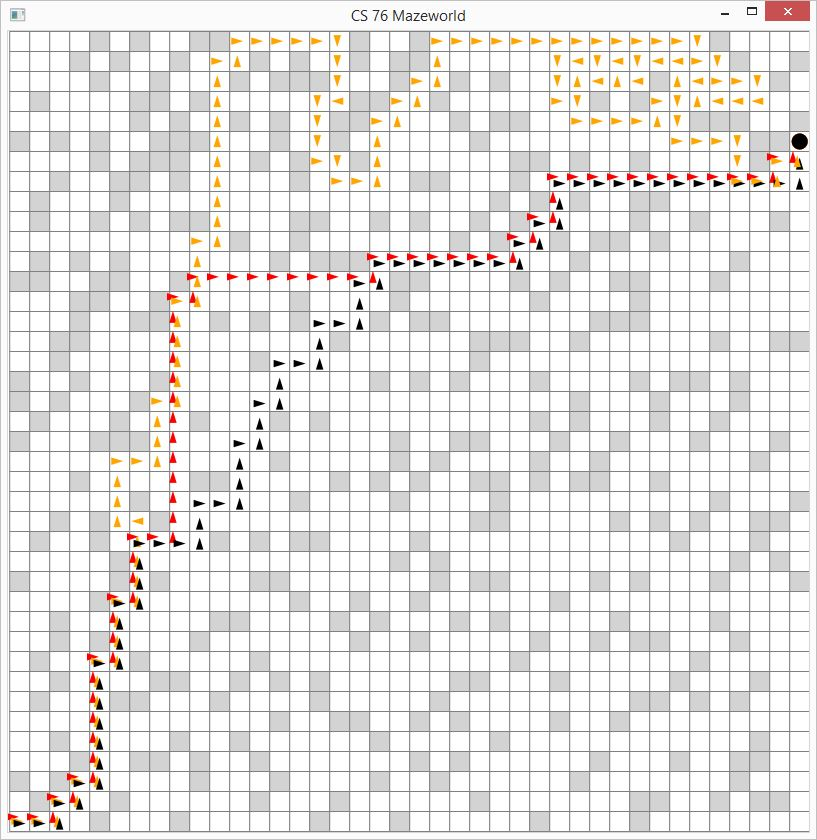
\includegraphics[width=0.927\textwidth]{s-1-1.JPG}
\caption{Searhing path of dfs(orange), bfs(red) and A*(black)}
\label{s-1}
\end{figure*}

The following output shows that, A* explored significantly less node than bfs, while the path length (cost) almost as less as bfs, while comparing to dfs.



\begin{lstlisting}[numbers=left]
BFS:  
  Nodes explored during search:  1064
  Maximum space usage during search 1099
  path length: 60
  
DFS:  
  Nodes explored during search:  399
  Maximum space usage during search 242
  path length: 242
  
A*:  
  Nodes explored during search:  79
  Maximum space usage during search 224
  path length: 72
\end{lstlisting}







\subsection{Discussion on cost and heuristic}
A* leverage both the cost (penalty) and the heuristic (search speed). Currently we use $f = h + g$ for priority, which seems quite a balanced solution. What happens if we go to extrem where the priority only related to $g$ or $h$? Or, is 50:50 the best choice for $f$?

Before I begin to discuss, I want to introduce a new kind of maze, where the obstacles can be crossed, while there is a certain amount of penalty. While I am first use Simplex Noise generate a maze, i replace the wall with number ranging from 1 to 10 to represent the weights. I use the following functions to differentiate nodes with different weights.
$$Grayscale = 255 - 255 \times weight / 20$$

Here I modify the expression of priority as following:
$$f = \alpha \cdot h + (1 - \alpha ) \cdot g$$
Then I vary $\alpha$ from 0 to 1, and observe their path length and cost. Figure \ref{s-2} shows the performance of different configuration. 
\begin{itemize}
  \item Red ($\alpha = 0.0$) is an extreme case when A* only considers the cost, and becomes uninformed search. (I think it act like Dijkstra Algorithm). Since we are using Manhattan distance and the goal is at top-right, every action of moving south or west is a compromise of cost, and neglecting of path length ( search speed).
  \item Brown ($\alpha = 1.0$) is another extreme case when A* only considers the heuristic, and becomes best-first search. We can observe that it totally neglect the cost/penalty, rushing to the goal in the simplest path.
\end{itemize}
Figure \ref{gh-plot} shows the change of path length and cost while varying $\alpha$. Depending on whether 

\begin{figure*}[!h]
\centering
\includegraphics[width=0.628\textwidth]{astar_alpha.eps}
\caption{Plot describes the relationship between cost, path length, and $\alpha$}
\label{gh-plot}
\end{figure*}

\begin{figure*}[!h]
\centering
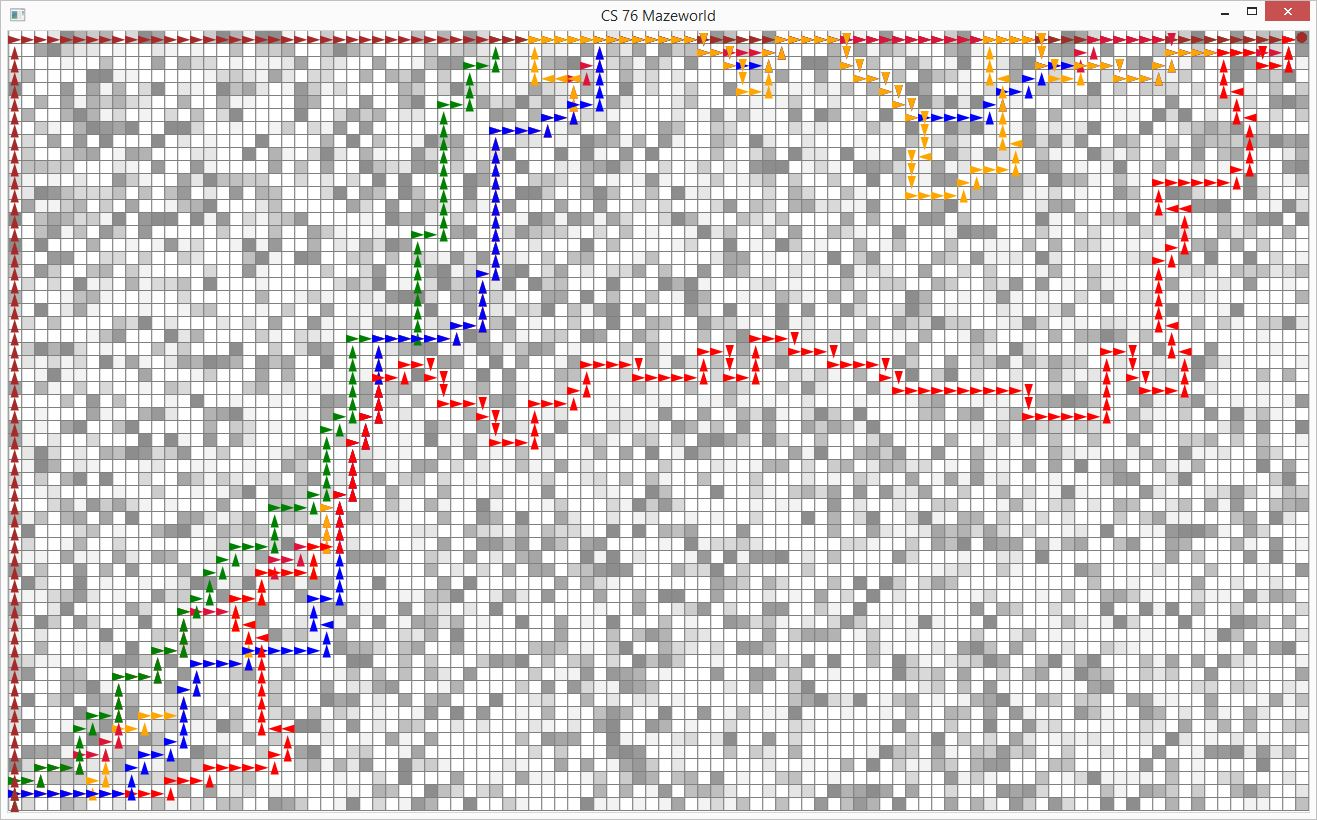
\includegraphics[width=1\textwidth]{s-2-1.JPG}
\caption{Varying the $\alpha$ in A* as 0.0 (red), 0.25 (orange), 0.5 (blue), 0.75 (crimson), 0.9 (green), 1.0 (brown)}
\label{s-2}
\end{figure*}

